\pgfplotsset{width=\textwidth,compat=1.3}
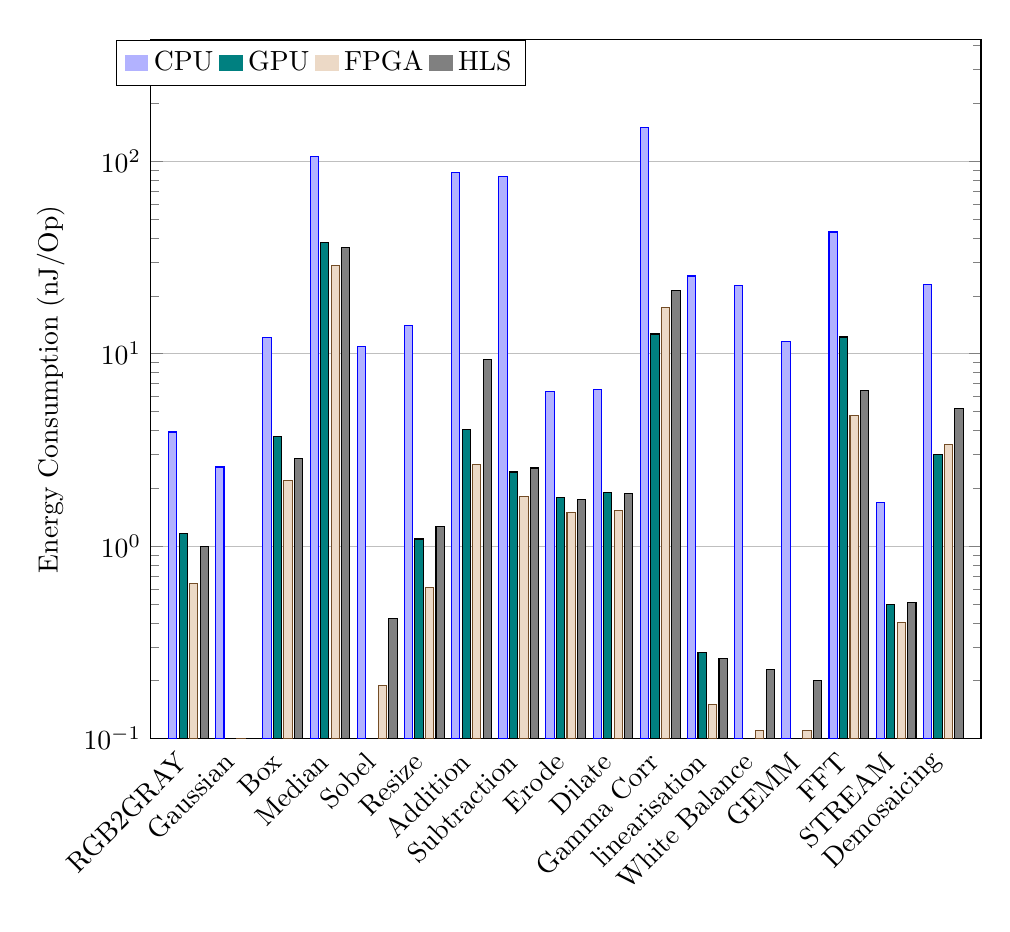
\begin{tikzpicture}
\begin{axis}[
    width  = \textwidth,
    major x tick style = transparent,
    ybar=2*\pgflinewidth,
    ymax=200,
    ymin=0.1,
    bar width=3pt,
    enlarge y limits={upper=0.15},
    legend image code/.code={\draw[#1, draw=none] (0cm,-0.1cm) rectangle (0.3cm,0.1cm);},
    ymode=log,
    ymajorgrids = true,
    ylabel = {Energy Consumption (nJ/Op)},
    symbolic x coords={RGB2GRAY, Gaussian, Box, Median, Sobel, Resize, Addition, Subtraction, Erode, Dilate, Gamma Corr, linearisation, White Balance, GEMM, FFT, STREAM, Demosaicing},
    xtick = data,
    xticklabel style={rotate=45, anchor=east},
    nodes near coords style={font=\tiny, anchor=west,rotate=90,inner xsep=0.5pt, black},
    enlarge x limits=0.05,
    legend cell align=left,
    legend style={at={(0.2049,0.9999)},anchor=north,legend columns=-1},
]
\addplot coordinates {
    (RGB2GRAY, 3.92) (Gaussian, 2.58) (Box, 12.19) (Median, 106.34)
    (Sobel, 10.96) (Resize, 14.08) (Addition, 87.77) (Subtraction, 83.19)
    (Erode, 6.34) (Dilate, 6.50) (Gamma Corr, 150.34) (linearisation, 25.35)
    (White Balance, 22.57) (GEMM, 11.52) (FFT, 42.87) (STREAM, 1.69)
    (Demosaicing, 22.98)
};

\addplot [fill=teal] coordinates {
    (RGB2GRAY, 1.16) (Gaussian, 0.10) (Box, 3.70) (Median, 37.65)
    (Sobel, 0.07) (Resize, 1.09) (Addition, 4.05) (Subtraction, 2.43)
    (Erode, 1.79) (Dilate, 1.91) (Gamma Corr, 12.66) (linearisation, 0.28)
    (White Balance, 0.10) (GEMM, 0.09) (FFT, 12.22) (STREAM, 0.50)
    (Demosaicing, 2.99)
};

\addplot coordinates {
    (RGB2GRAY, 0.64) (Gaussian, 0.06) (Box, 2.19) (Median, 28.76)
    (Sobel, 0.19) (Resize, 0.61) (Addition, 2.65) (Subtraction, 1.82)
    (Erode, 1.49) (Dilate, 1.54) (Gamma Corr, 17.44) (linearisation, 0.15)
    (White Balance, 0.11) (GEMM, 0.11) (FFT, 4.78) (STREAM, 0.40)
    (Demosaicing, 3.36)
};

\addplot coordinates {
    (RGB2GRAY, 1.00) (Gaussian, 0.08) (Box, 2.85) (Median, 35.65)
    (Sobel, 0.42) (Resize, 1.27) (Addition, 9.34) (Subtraction, 2.55)
    (Erode, 1.75) (Dilate, 1.87) (Gamma Corr, 21.26) (linearisation, 0.26)
    (White Balance, 0.23) (GEMM, 0.20) (FFT, 6.42) (STREAM, 0.51)
    (Demosaicing, 5.18)
};

\legend{CPU, GPU, FPGA, HLS}
\end{axis}
\end{tikzpicture}